\begin{minipage}[b]{6cm}
        \scshape%
        Example University
\end{minipage}\hfill
\ifexamempty
    % for backup exams (without qr code)
    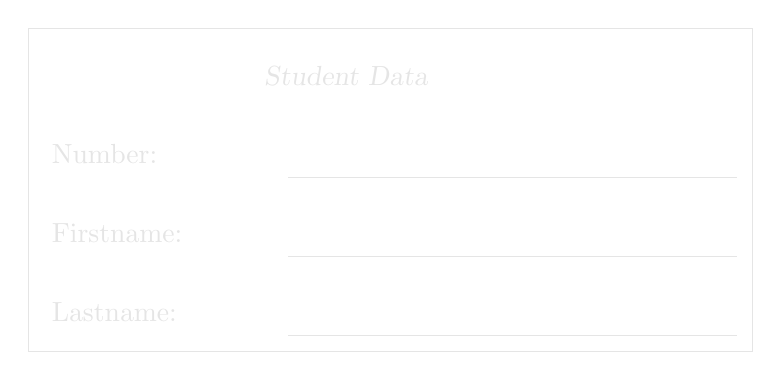
\begin{tikzpicture}
    \draw[draw = lightgray!40] (0, 0) rectangle (9.2,4.1);
    \draw (5,3.5) node[text width=4cm] {\textsl{\textcolor{lightgray!40}{Student Data}}};
    \draw (1.3,2.5) node[text width=2cm, align=left] {\textcolor{lightgray!40}{Number:}};
    \draw[draw = lightgray!40] (3.3,2.2) -- (9.0, 2.2);
    \draw (1.3,1.5) node[text width=2cm, align=left] {\textcolor{lightgray!40}{Firstname:}};
    \draw[draw = lightgray!40] (3.3,1.2) -- (9.0, 1.2);
    \draw (1.3,0.5) node[text width=2cm, align=left] {\textcolor{lightgray!40}{Lastname:}};
    \draw[draw = lightgray!40] (3.3,0.2) -- (9.0, 0.2);
    \end{tikzpicture}
\else
    \begin{minipage}{2cm}
        % Json is also supported:
%        \vspace{-0.5cm}
%        \qrcode[height=2cm]{\{"Mat" :\matno,"No" :\sortindex\}}
        \qrcode[height=1.5cm]{\sortindex}
    \end{minipage}
    \begin{minipage}{2cm}
        \raggedleft
        \huge \sortindex % for sorting exams alphabetically
    \end{minipage}\hfill
\fi

\normalfont
\thispagestyle{headandfoot}
\firstpagefooter{}{}{} % for extra space

\ifprintanswers
\else
\ifexamempty
\else
\begin{framed}
    \textbf{\lastname, \firstname} (\no) \hfill \room, \seat~(\seatindex)
\end{framed}
\fi
\fi

Change the definition of ifexamempty to disable individualized exams.

\vspace*{4mm}
% \begin{tabularx}{\textwidth}{X}
% \hhline{-}\\
% 
% \end{tabularx}

\hrule


\vspace{\baselineskip}

\begin{center}
    \ifnum \numpoints < 100
        \htword{$\Sigma$}
    \else
        \htword{\hspace{0.5mm}Summe\hspace{0.5mm}} % wider sum field
    \fi
    \cellwidth{.8cm}
    
    \usetikzlibrary{calc}
    \hsword{
        Achieved
        \begin{tikzpicture}[overlay]
            \def\base{
                -\numquestions*\baselineskip*3*.5-\baselineskip*4.53*.5+\baselineskip*4+44.2,0.51
            }
            \coordinate (first_dashed) at ($(\base)+(3*1.236/3+0*1.236-2.572,-.7)$);
            \draw[gray, dashed] (first_dashed) -- ++(0,-.73); % first dashed line
            \foreach \x in {1,...,\numquestions} {
                \foreach \y in {1,2} {
                    \draw[gray, dashed] ($(\base)+(\y*1.236/3+\x*1.236-2.572,0)$) -- ++(0,-.73);
                    \draw[gray, dashed] ($(\base)+(\y*1.236/3+\x*1.236-2.572,-.7)$) -- ++(0,-.73);
                }
                \draw[gray, dashed, line width=0.35mm] ($(\base)+(2*1.236/3+\x*1.236-2.572,-.62)$) -- ++(0,-.13);
                \draw[gray, dashed] ($(\base)+(3*1.236/3+\x*1.236-2.572,-.7)$) -- ++(0,-.73);
            }
            \ifnum \numpoints < 100
            \coordinate (last_dashed) at ($(\base)+(3*1.236/3+\numquestions*1.236-1.342,-.7)$);
            \draw[gray, dashed] ($(\base)+(1*1.336/3+\numquestions*1.236-1.372,0)$) -- ++(0,-.73);
            \draw[gray, dashed] ($(\base)+(1*1.336/3+\numquestions*1.236-1.372,-.7)$) -- ++(0,-.73);
            \draw[gray, dashed] ($(\base)+(2*1.336/3+\numquestions*1.236-1.372,0)$) -- ++(0,-.73);
            \draw[gray, dashed] ($(\base)+(2*1.336/3+\numquestions*1.236-1.372,-.7)$) -- ++(0,-.73);
            \draw[gray, dashed, line width=0.35mm] ($(\base)+(2*1.336/3+\numquestions*1.236-1.372,-.62)$) -- ++(0,-.13);
            \draw[gray, dashed] (last_dashed) -- ++(0,-.73); % last dashed line
            \else
            \coordinate (last_dashed) at ($(\base)+(3*1.336/3+\numquestions*1*1.236-1.372,-.7)$);
            \draw[gray, dashed] ($(\base)+(1*1.336/3+\numquestions*1.236-1.372,0)$) -- ++(0,-.73);
            \draw[gray, dashed] ($(\base)+(1*1.336/3+\numquestions*1.236-1.372,-.7)$) -- ++(0,-.73);
            \draw[gray, dashed] ($(\base)+(2*1.336/3+\numquestions*1*1.236-1.372,0)$) -- ++(0,-.73);
            \draw[gray, dashed] ($(\base)+(2*1.336/3+\numquestions*1*1.236-1.372,-.7)$) -- ++(0,-.73);
            \draw[gray, dashed] ($(\base)+(3*1.336/3+\numquestions*1*1.236-1.372,0)$) -- ++(0,-.73);
            \draw[gray, dashed] (last_dashed) -- ++(0,-.73); % last dashed line
            \fi
            % eine Zellbreite ist 0,44
            \node at ($(first_dashed) + (-0.7, -0.48)$) {\includegraphics{aruco_bottom_left.png}}; % bottom right corner must be aligned with table, distance one cell width
            \node at ($(last_dashed) + (0.7, 1.91)$) {\includegraphics{aruco_top_right.png}}; % upper left corner must be aligned with table, distance one cell width
            \node at ($(last_dashed) + (0.7, -0.48)$) {\includegraphics{aruco_bottom_right.png}}; % bottom left corner must be aligned with table, distance one cell width
            \node at ($(first_dashed) + (-0.7, 2.39)$) {\includegraphics{aruco_top_left.png}}; % bottom right corner must be aligned with table, distance one cell width
        \end{tikzpicture}
    }
    \setcounter{numquestions}{0} % for personalized exams
    \partialgradetable{myrange}[h][questions]
    \setcounter{numpoints}{0} % hack; needed for correct width of sum if exams are personalized
\end{center}


\setcounter{page}{1}

